\chapter{Objetivos}\label{cap.objetivos}
\hspace{1cm} Una vez introducidas las motivaciones que me han llevado a hacer este tfg y expuestos los conceptos mas importantes que se deben saber para comprender la totalidad del trabajo, en este capitulo se van a exponer los diferentes problemas que se abordaran a lo largo de la memoria, los requisitos para poder abordar estos problemas y por último la metodología y el plan de trabajo que se ha seguido. 


\section{Problemas a abordar}
\hspace{1cm} El objetivo principal de este trabajo es la creación de un sistema  que permita el funcionamiento de un dron completamente autónomo con esto queremos decir que despegue de forma controlada, siga una ruta previamente establecida y aterrice tambien de forma controlada. Para la parte de enrutamiento el drone ha de conocer en todo momento su posición en
el entorno mediante técnicas de visión por computador basadas en marcadores visuales
artificiales, mientras que para el despegue y aterrizaje controlados debe reconocer las balizas por visión cuya posición es desconocida. 

\hspace{1cm} Conociendo el objetivo principal este se ha desglosado en varios subobjetivos para poder abordarlo correctamente:

\begin{enumerate}
	\item{\textbf{Utilización de la herramienta Visual States:} La cual nos permitirá crear la jerarquía necesaria para poder pasar de un estado a otro mediante transiciones y así poder dividir nuestro programa e ir mejorándolo e implementando las nuevas creaciones sin tener que modificar las otras partes, además de esto creará una interfaz gráfica en la cual representa el comportamiento del robot gráficamente y así se puede distinguir el estado en el que se encuentra. Esta representación gráfica permite un mayor nivel de abstracción para el usuario, ya que solo tiene que preocuparse por programar las acciones actuales del robot y seleccionar qué componentes puede necesitar de la interfaz del robot.}
	\item{\textbf{Adaptación e integración del componente Slam-Visualmarkers:} Como nadie había utilizado la herramienta de Visual States integrando el componente de slam-visualmakers hemos tenido que ajustar este componente e introducirlo por pasos para poder finalmente conseguir su correcto funcionamiento en la misma.}
	\item{\textbf{Recodificación e integración del aterrizaje visual:} Ya que este estaba creado a partir de una posición dada en altura y contaba con temporizadores y una maquina virtual de estados. Por esto se ha modificado para poder integrarlo en nuestro sistema de navegación y además a partir de este se ha creado el propio sistema de despegue controlado.}
	\item{\textbf{Desarrollo de dos componentes de navegación basados en la posición absoluta del drone:} Ambos serán controles de pilotaje aplicados sobre las posiciones obtenidas por el componente slam-visualmarkers, la diferencia radicara en que a uno le estableceremos una serie de puntos o balizas a los cuales debe de llegar mientras que el otro deberá seguir una ruta.}
	\item{\textbf{Validación experimental en entorno simulado Gazebo:} Se creará un mundo tridimensional en el que se realizarán las pruebas pertinentes para determinar la robustez
del sistema en conjunto. Se examinará para ambos componentes de navegación el error de la estimación de posición y cómo este puede afectar al sistema de pilotaje del cuadricóptero, ademas se comparara con anteriores sistemas de pilotajes y se verán las posibles mejoras. También se calculará el error producido en la estimación de posición por el componenete Slam-Visualmakers.}
\end{enumerate}


\section{Requisitos}
\hspace{1cm} Una vez descritos todos los objetivos, lo siguiente es nombrar los requisitos que va a satisfacer la aplicación que hemos desarrollado:

\begin{itemize}
		\item El algoritmo funcionará en la plataforma de desarrollo JdeRobot-5.6.3.
		\item El sistema se ejecutara en el entorno GNU/Linux Ubuntu 16.04.
		\item La aplicación se ejecutara en el simulador Gazebo con la utilización del robot Ar.Drone.
		\item El sistema debe ser exportable a cualquier escenario que sea un espacio simulado controlado y contenga marcadores AprilTags con posiciones conocidas.
		\item Para la autolocalización, el sistema sólo puede depender de las imágenes servidas por la cámara del drone y utilizando el componente Slam-Visualmarkers.
		\item El control de navegación mediante el pilotaje debe ser suave para no perder los marcadores y balizas, pero tambien robusto, fluido y vivaz para que el drone se mueva de forma ágil y veloz por el entorno y sus rutas establecidas.
		\item Programado en Python 2.7.
\end{itemize}


\section{Metodología}
\hspace{1cm} Al tratarse de un trabajo de integración y desarrollo software el modelo de trabajo que se ha seguido ha sido el de desarrollo en espiral. Este modelo nos ha permitido trabajar de forma progresiva, es decir, empezando por las partes mas sencillas y a medida que las íbamos logrando ir avanzando hasta las mas complejas. Para ello la forma de conseguirlo fue mediante la marcación de hitos o pautas a alcanzar que se revisaban periódicamente mediante reuniones con el tutor, de esta forma se analizaban si se había conseguido llegar al resultado esperado en cada etapa y así poder pasar al siguiente objetivo analizando para ello las posibles rutas que se podían seguir según la toma de decisiones y la evaluación de riesgos. Cuando se alcanzaba un objetivo lo suficientemente importante se creaba una entrada en el cuaderno de bitácora de JdeRobot, el cual es público y nos ha servido para llevar un seguimiento de las áreas realizadas y como punto de comunicación con el tutor para saber las dificultades que teníamos y como poder solucionarlas.  

\hspace{1cm} En el siguiente enlace del mediawiki o cuaderno de bitácora mencionado anteriormente se pueden encontrar desde fotos y videos de la practica final como resultados y pasos iniciales que se hicieron para adentrarse en el mundo de la programación de robots y drones \href{http://jderobot.org/Jsaizc-tfg}{http://jderobot.org/Jsaizc-tfg}. Tambien se puede visitar el código de todas estas etapas que se observan en el mediawiki, este es de acceso público en GitHub \href{https://github.com/RoboticsURJC-students/2017-tfg-jesus-saiz}{https://github.com/RoboticsURJC-students/2017-tfg-jesus-saiz}.

\begin{figure}[H]
	\begin{center}
		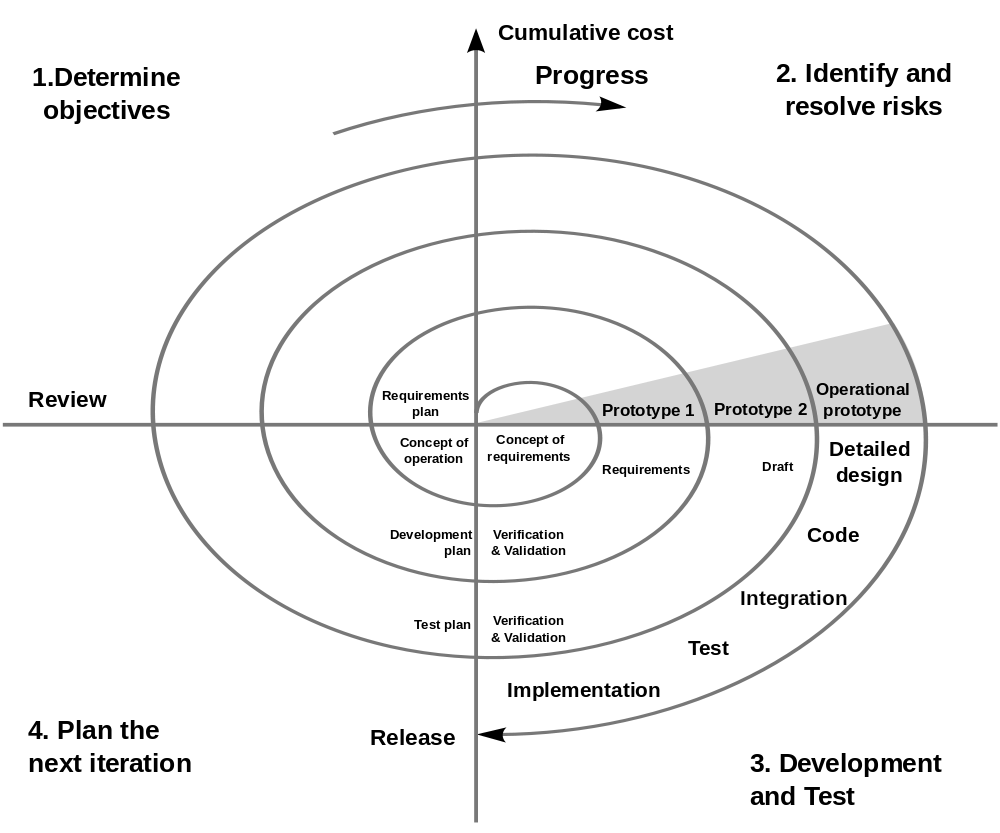
\includegraphics[width=0.6\textwidth]{imag/IMG17.png}
				\caption{Representación del desarrollo en espiral.} 
	\label{fig:Desarrollo en espiral.}	
	\end{center}
\end{figure}


\section{Plan de trabajo}
\hspace{1cm} Para conseguir la metodología de trabajo expuesta anteriormente se ha seguido una planificación dividida en las siguientes fases:

\begin{itemize}
	\item \textbf{Programación en Python:} Necesaria para poder entender el código anterior en el que me he basado y crear el mio propio. Con el conocimiento de c/c++ y una serie de guías de ayuda fue el  primer paso de aprendizaje.
	\item \textbf{Formación en JdeRobot:} Había que comprender el funcionamiento de la plataforma y saber todas las herramientas con las que contaba para saber en que te podías basar y que era lo que tenias que desarrollar tu mismo. Para ello se realizaron una serie de programas simples en los cuales trabajabas con distintos robots y con diferentes herramientas, teniendo así los primeros contactos con programación de robots simulados y reales.
	\item \textbf{Familiarización con Gazebo:} El simulador utilizado preferentemente en JdeRobot, en el hubo que crear el entorno de simulación sobre el cual se basaría el programa de vuelo del drone.	
	\item \textbf{Estudio y desarrollo del interfaz gráfico:} El programa se ha desarollado sobre la aplicación Visual States, la cual he tenido que aprender para conseguir introducir todas las etapas y que funcionase correctamente.
	\item \textbf{Aprendizaje e integración del componente de autolocalización:} Necesario para conocer el funcionamiento de este componente y poder manejar los parámetros y las balizas con las que trabaja, para así poder conseguir una correcta autolocalización del drone y tambien obtener los errores de la herramienta y extraerlos de los errores de pilotaje.
	\item \textbf{Adaptación y desarrollo del control de aterrizaje:} Para poder adaptarlo a la aplicación de Visual States y a su vez crear un propio sistema de despegue del drone.
	\item \textbf{Desarrollo del algoritmo para el control de pilotaje:} De dos formas diferentes, por un lado el algoritmo de seguimiento de puntos y por otro lado el de seguimiento de trayectorias. Ambos capaces de gobernar el movimiento del drone para seguir las rutas en 3D. 
	\item \textbf{Validación experimental en entornos simulados:} Para comprobar y validar el correcto funcionamiento de las fases anteriores se realizaron una serie de experimentos en entornos simulados, con estas pruebas se detectaron posibles comportamiento erróneos que corrigiéndolos se consiguió estabilidad en el sistema y una posible viabilidad en entornos reales.   
\end{itemize}
